\begin{frame}
  \frametitle{The CLAS12 Drift Chamber}
  \begin{itemize}
    \item Subsystem of the CLAS12 particle detector
      \begin{itemize}
        \item Electron beam hits target inside the detector's center
        \item Drift Chamber (DC) is used to measure the results
          (particle momentum)
      \end{itemize}
    \item Hierarchical arrangement of multiple wires grouped together
      as wire chambers
      \begin{itemize}
        \item Wires are used to detect particle presence
        \item Particle hits wire \(\rightarrow\) wire gets activated
      \end{itemize}
  \end{itemize}
\end{frame}

\begin{frame}
  \frametitle{The CLAS12 Drift Chamber}
  \begin{figure}
    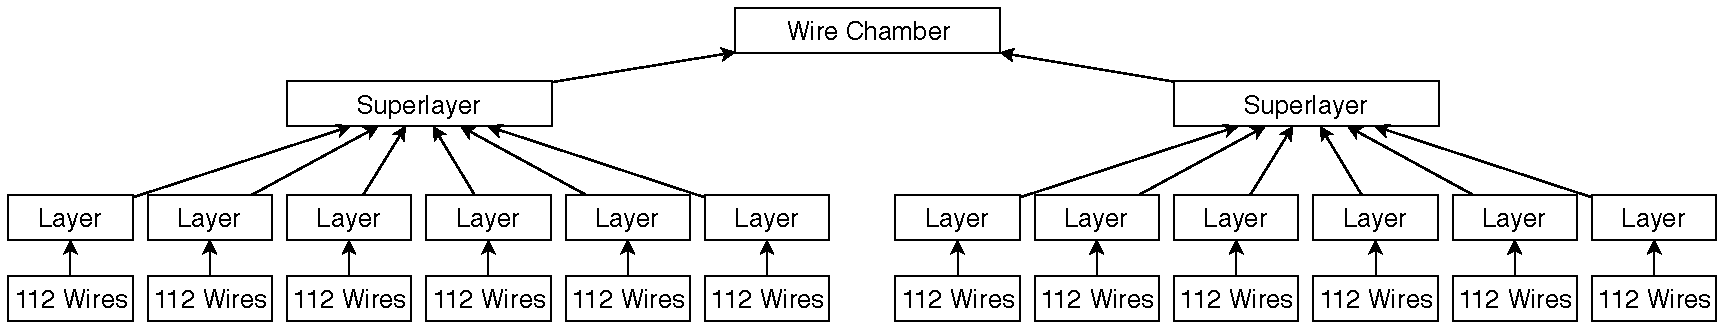
\includegraphics[width=\textwidth]{../figures/wire_chamber}
    \caption{The hierarchical structure of a single wire chamber.}
  \end{figure}
\end{frame}

\begin{frame}
  \frametitle{Drift Chamber Faults}
  \begin{itemize}
    \item Drift chamber operates under extreme conditions
      \begin{itemize}
        \item Huge amounts of radiation
        \item Components can get damaged during an experiment
        \item Single wires or collections thereof stop working
      \end{itemize}
    \item Wire activations can be visualized as heatmaps
      \begin{itemize}
        \item Easier to detect faults
      \end{itemize}
  \end{itemize}
\end{frame}

\begin{frame}
  \frametitle{Dead Wire}
  \begin{figure}
    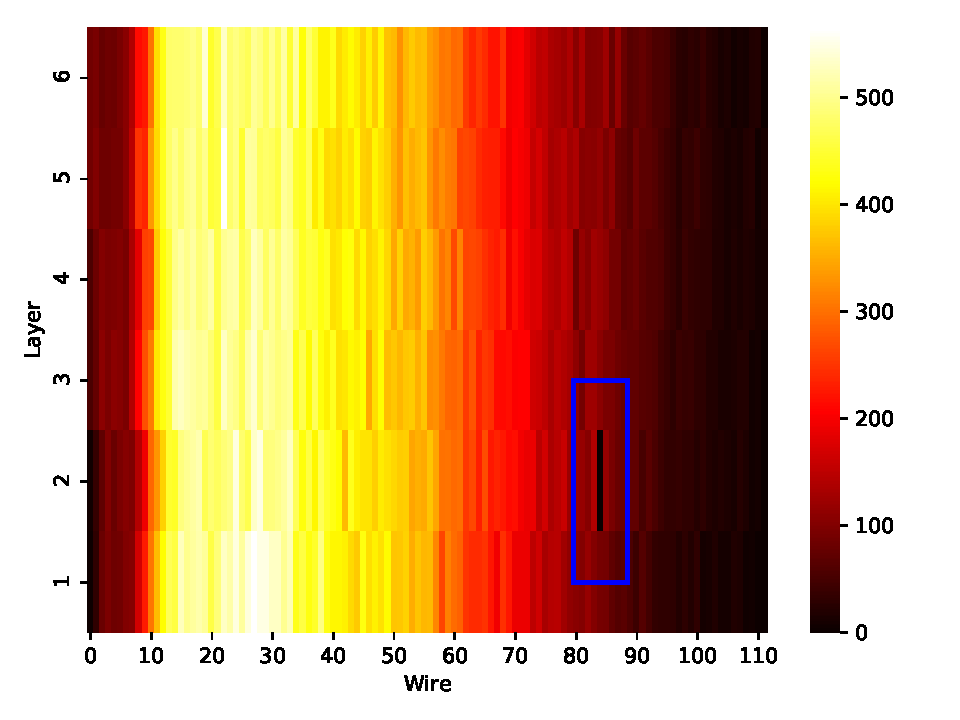
\includegraphics[width=.85\textwidth]{../figures/dead_wire}
  \end{figure}
\end{frame}

\begin{frame}
  \frametitle{Dead Pin}
  \begin{figure}
    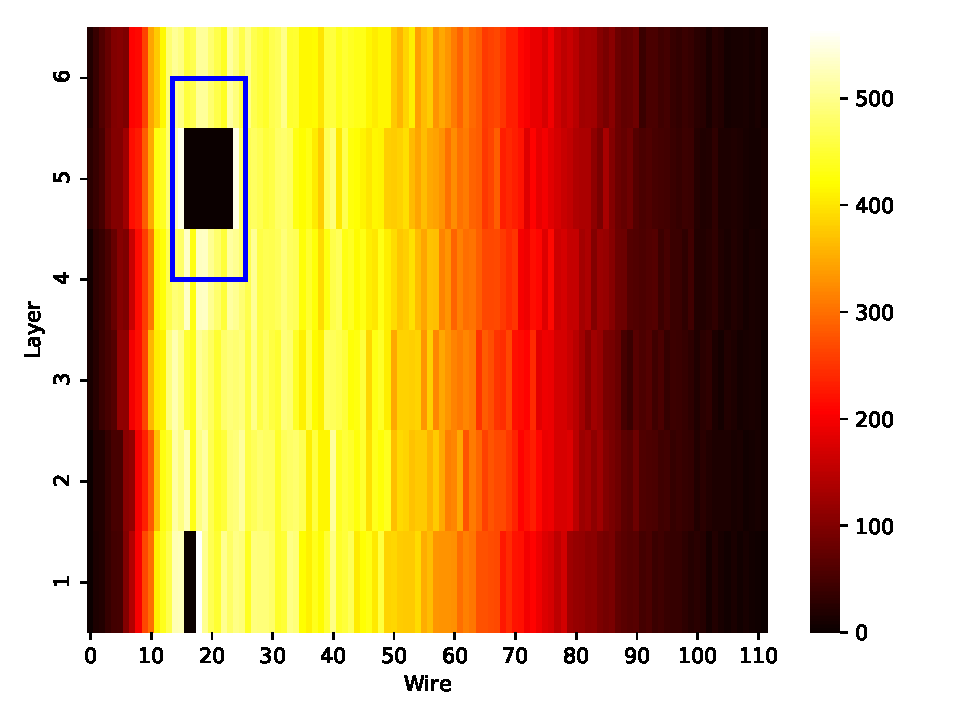
\includegraphics[width=.85\textwidth]{../figures/dead_pin}
  \end{figure}
\end{frame}

\begin{frame}
  \frametitle{Dead Connector}
  \begin{figure}
    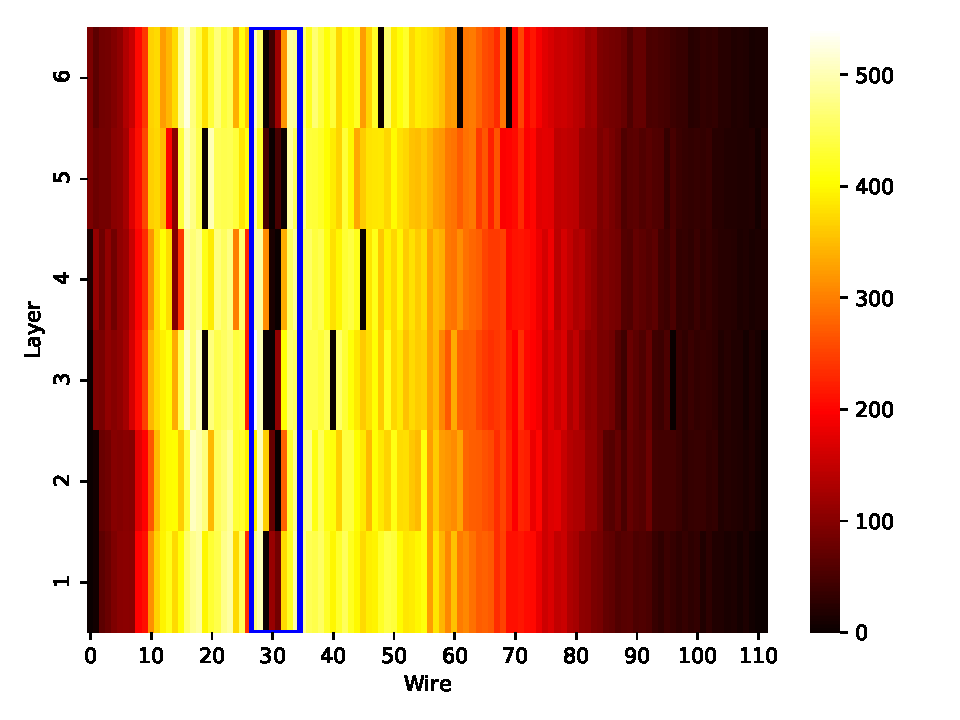
\includegraphics[width=.85\textwidth]{../figures/dead_connector}
  \end{figure}
\end{frame}

\begin{frame}
  \frametitle{Dead Fuse}
  \begin{figure}
    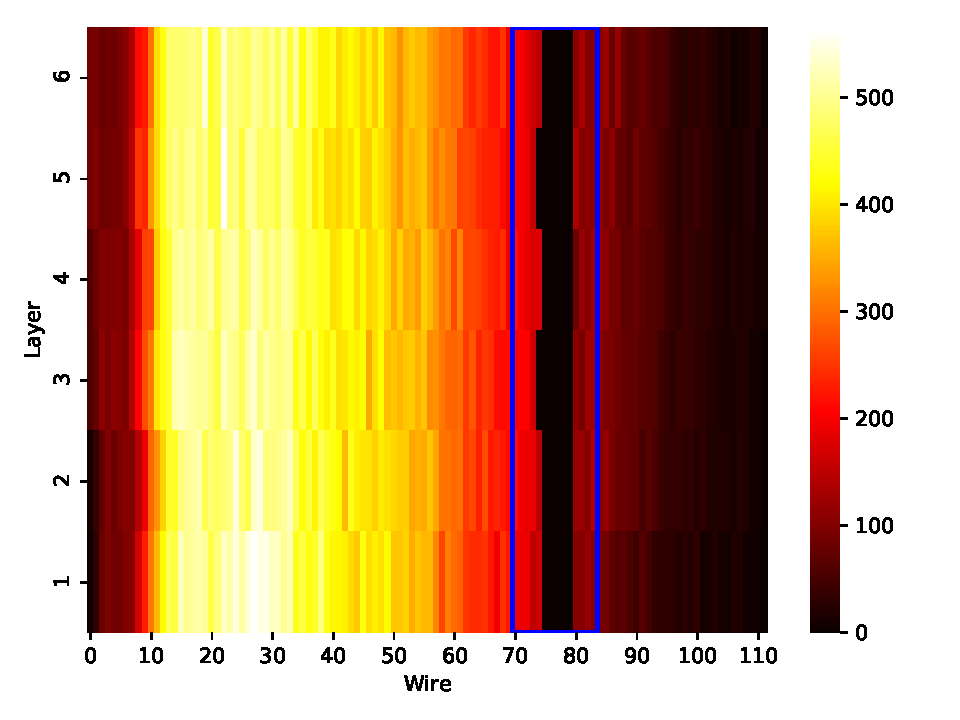
\includegraphics[width=.85\textwidth]{../figures/dead_fuse}
  \end{figure}
\end{frame}

\begin{frame}
  \frametitle{Dead Channel}
  \begin{figure}
    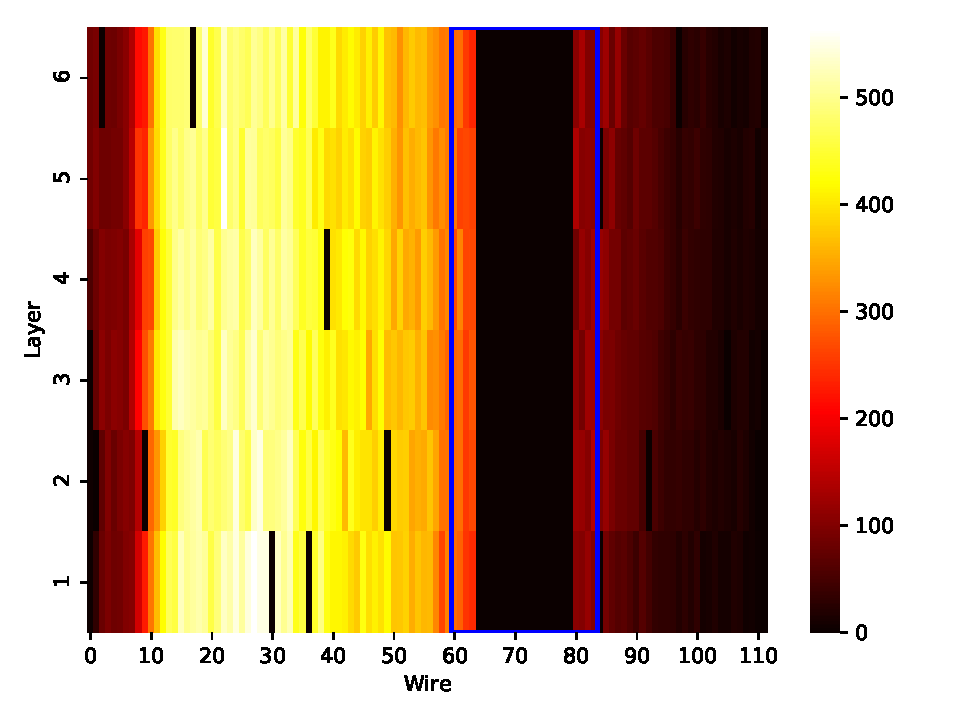
\includegraphics[width=.85\textwidth]{../figures/dead_channel}
  \end{figure}
\end{frame}

\begin{frame}
  \frametitle{Hot Wire}
  \begin{figure}
    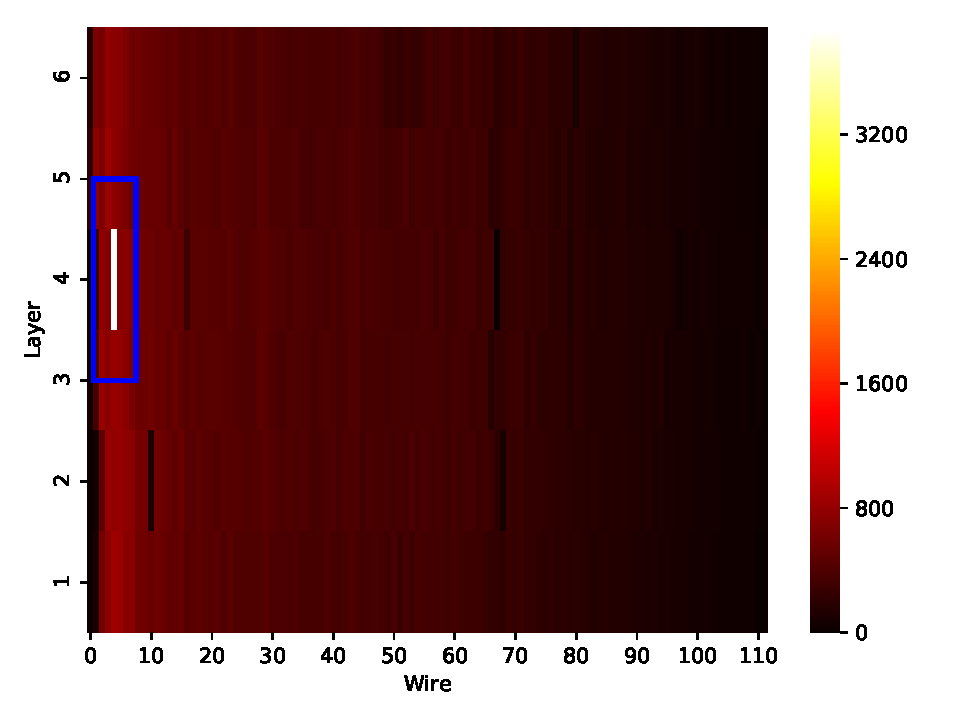
\includegraphics[width=.85\textwidth]{../figures/hot_wire}
  \end{figure}
\end{frame}
